% ----------------------------------------------------------
% Modelagem do Projeto
% ----------------------------------------------------------
\chapter{Modelagem do Projeto} \label{cha:modelagem}

\section{Levantamento de Requisitos}

\subsection{Requisitos Funcionais}
  Abaixo são listados os requisitos funcionais do sistema: 

  \begin{enumerate}
    \item \textbf{Fornecimento de localização de veículos}: Fornecer informações de localização dos veículos do sistema no momento solicitado.
    \item \textbf{Catálogo de linhas disponíveis no Sistema}: Listar as linhas disponíveis no sistema.
    \item \textbf{Catálogo das paradas de ônibus}: Listar as paradas disponíveis no sistema e as linhas que estão disponíveis em cada uma delas.
    \item \textbf{Avaliação de entidades do sistema}: Registar avaliações dos usuários sobre paradas e veículos do sistema de transporte público.
    \item \textbf{Gerenciamento de usuários e autenticação}: Listar histórico de operações do usuário e ranking de usuários cadastrados.  
  \end{enumerate}

\subsection{Requisitos Não Funcionais}
  Abaixo são listados os requisitos não funcionais do sistema:

  \begin{enumerate}
    \item \textbf{Escalável e de alta disponibilidade}: Deve ser facilmente escalável para atender o aumento repetino de demanda ao mesmo 
    tempo que mantem-se sempre disponível.
    \item \textbf{Baixa carga de trabalho de Infra}: A baixa carga carga baixa de trabalho de infra pode ajudar na evolução da plataforma. 
    \item \textbf{API deve se simples e flexível}: Para ser atrativa ao uso de desenvolvidores a api deve ser bem documentada e flexível.
  \end{enumerate}

\section{Diagramas de casos de uso} \label{sec:modelagem:casos}

O diagrama de caso de uso desenvolvido mostrado na figura \ref{fig:uml_caso_uso} descreve as possíveis interações do usuário através da ferramenta.

\begin{figure}[H]
  \caption{\label{fig:uml_caso_uso}Diagrama UML de Casos de Uso}
  \centering
  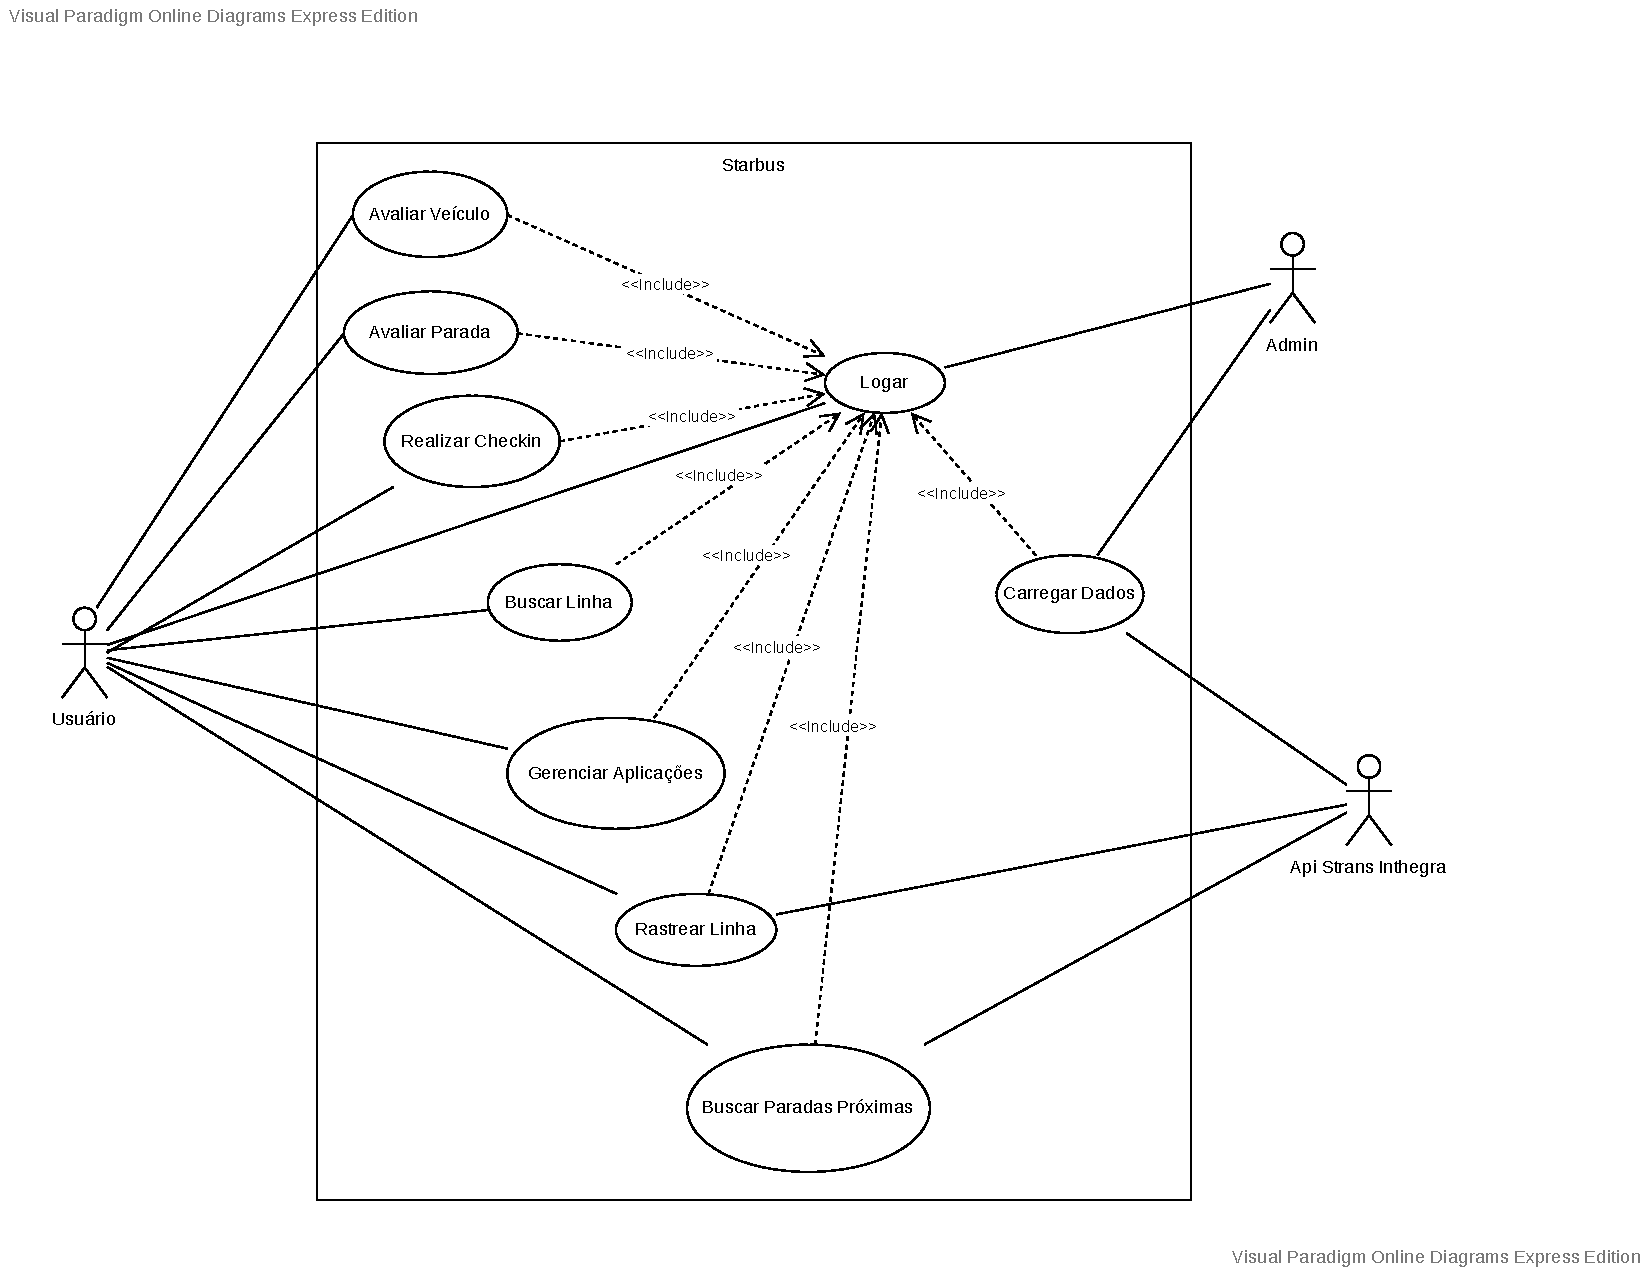
\includegraphics[scale=0.7]{imagens/usecase-sb.pdf}
  \legend{Caso de uso Starbus}
\end{figure}

O diagrama acima expressa os seguintes casos de uso:

\begin{enumerate}
  \item \textbf{Logar}: Ação de identificar-se como usuário para permitir a utilização dos recursos 
  da plataforma representados pelos casos de uso seguintes. Para manter a credibiliade das 
  informações fornecidas pelo usuários é essencial a identificação de cada fornecedor.  
  \item \textbf{Carregar Dados}: Usuário adminnistrador pode carregar as informações de linhas 
  e paradas a partir da API Strans Inthegra. Essa ação será executada sempre que houver 
  necessidade de atualizar a base do Starbus com novas informações da API Strans Inthegra.
  \item \textbf{Avaliar Veículo}: Usuário devidamente identificado publica sua opinião sobre 
  o veículo que utilizado em aspectos como acessibilidade, estado de conservação, lotação e conforto;
  \item \textbf{Avaliar Parada}: Usuário devidamente identificado publica sua opinião sobre 
  a parada de ônibus em aspectos como acessibilidade, estado de conservação, movimentação e 
  conforto;
  \item \textbf{Realizar Checkin}: Usuário devidamente identificado indica que no momento 
  econtra-se em uma devida parada de ônibus ou veículo; Essa informação pode ser útil para levantar
  a lotação dos veículos e das paradas de ônibus.  
  \item \textbf{Buscar Linha}: Usuário fornece um código ou um termo para pesquisa que é usado 
  para encontrar uma linha que ele deseja detalhes, como itinerário e localização dos veículos;
  \item \textbf{Gerenciar Aplicações}: Um usuário pode ter várias aplicações, aqui ele pode gerencia-las;
  \item \textbf{Rastrear Linha}: Tendo um identificador de uma linha, que pode ser recuperado 
  no caso de uso anterior, consulta a localização dos veículos dessa linha em tempo real com dados 
  fornecidos pela Api Strans Inthegra;
  \item \textbf{Buscar Paradas Próximas}:Usuário fornece uma localização, que pode ser a sua atual 
  ou de um ponto específico que pode quer chegar, a plataforma retorna todas as paradas próximas 
  aquele ponto, com os dados da parada inclusive a avaliação dos usuários sobre a parada;
\end{enumerate}

\section{Diagramas de classe} \label{sec:modelagem:classe}

O modelo de dados da aplicação apresentado na Figura \ref{fig:diagram_class}, onde é apresentado um diagrama 
UML de classes do projeto model.

\begin{figure}[H]
  \caption{\label{fig:diagram_class}Diagrama UML de Casos de Uso}
  \centering
  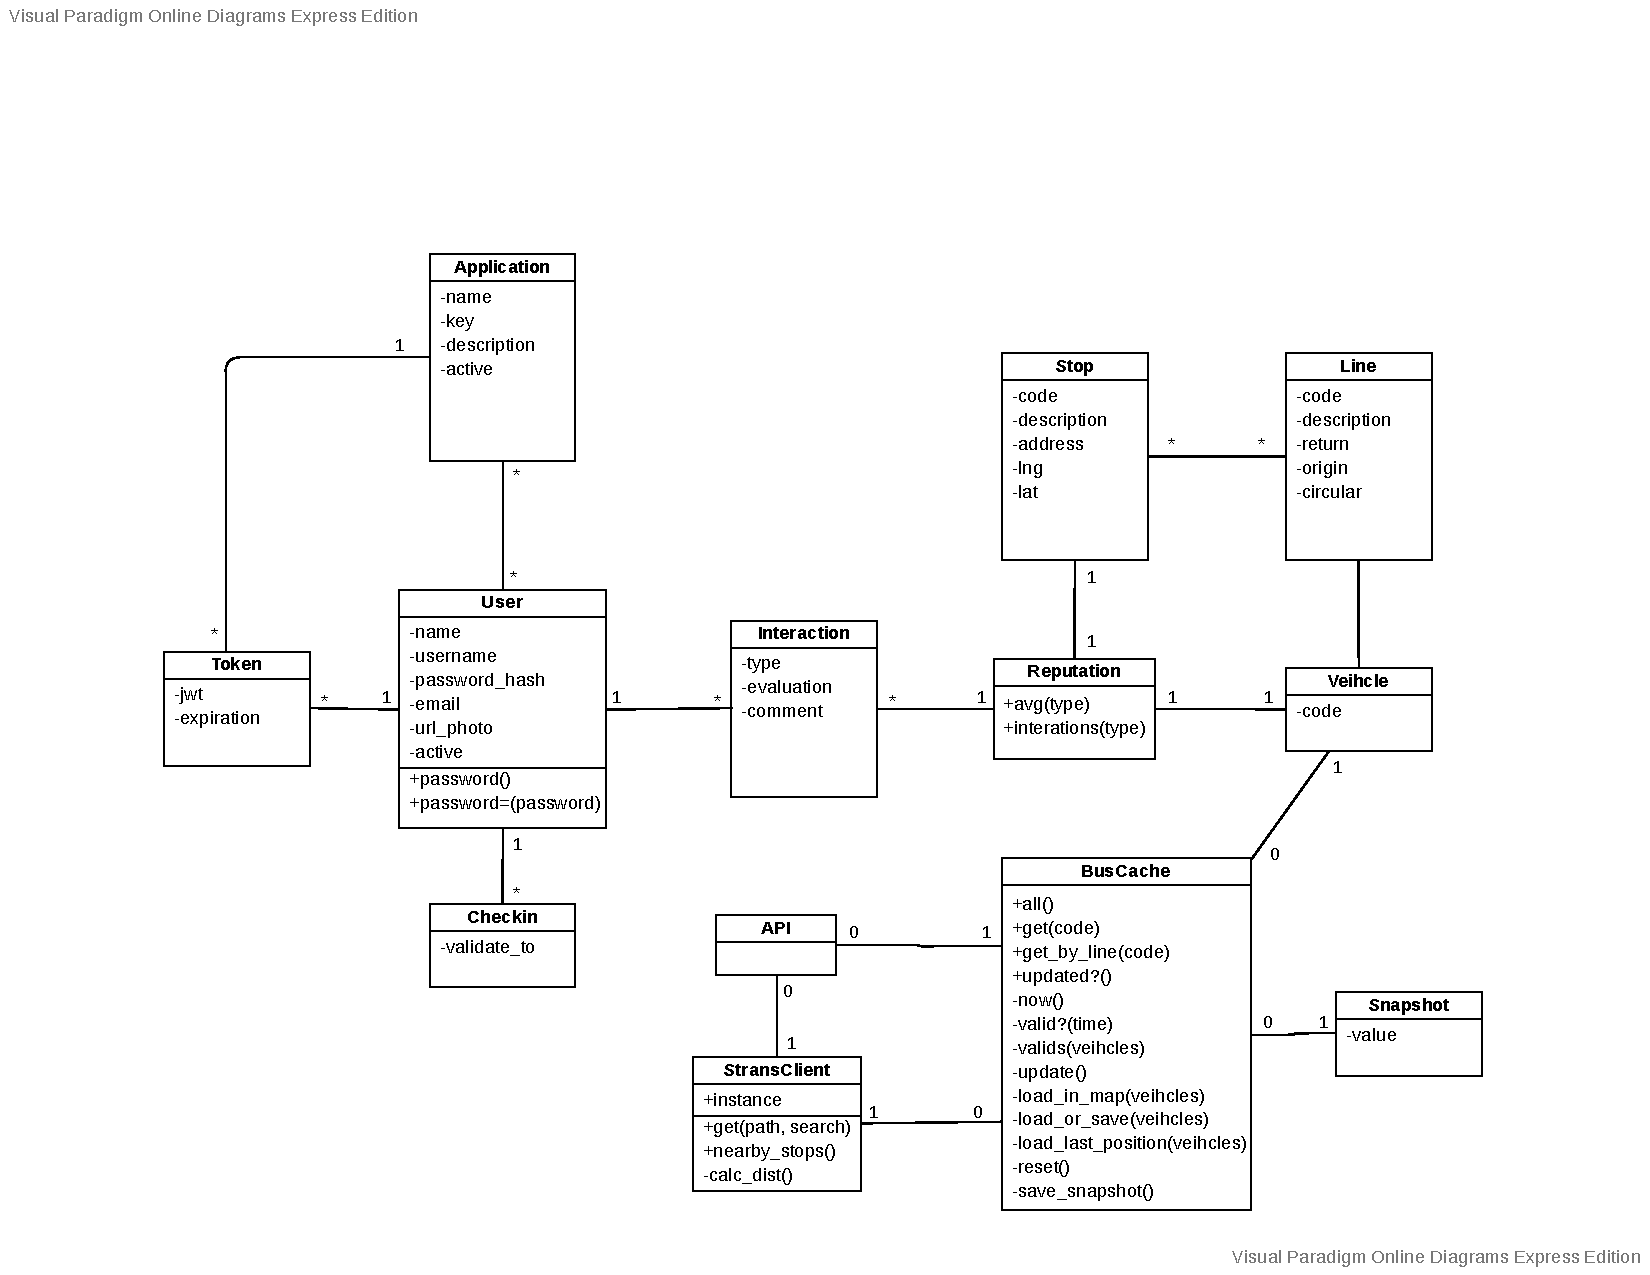
\includegraphics[scale=0.6]{imagens/diagramclass-sb.pdf}
\end{figure}

\begin{lista}
  \item \textbf{Application}: Representação de uma entidade que gera ou consome dados do starbus, sendo
  que esta pertence a um usuário e pode ter diversos usuários associados a ela. 
  \item \textbf{User}: A identidade de um usuário do sistema que acessa a plataforma por 
  meio de uma aplicação. Todo usuário possui  username e password que são utilizados para a autenticação no sistema, 
  somente após a autenticação é possível que um usuário possa consumir ou produzir informações para a plataforma.
  \item \textbf{Token}: Identidade Temporaria para que um usuário logado possa interajir com a plataforma. O token é 
  gerado no momento do login e armazenado para ser validado posteriormente a cada iteração com a plataforma. 
  Um Token tem um ciclo de vida bem definido e curto.
  \item \textbf{Checkin}: Um usuário pode notificar a sua localização em um determinado instante, pode ser uma parada 
  de ônibus ou em um veículo específico, tal informação poderá ser utilizado pela plataforma para verificar as condições
  de lotação das paradas ou dos veículos em determinado momento. O Checkin representa essa informação e está diretamente
  relacionado ao caso de uso cinco, Realizar Chekin.
  \item \textbf{Interaction}: Dados e comportamento dos casos de uso de Avaliar Veículo e Avaliar Parada, que são 
  sumarizados, na classe seguinte Reputation;
  \item \textbf{Reputation}: Sumarização de todas as avaliações realizadas por usuários a uma entidade do sistema de 
  transporte público, representando a reputação de cada veículo ou parada do sistema a ela associada.
  \item \textbf{Stop}: Parada de ônibus, com seu indentificador, endereço e localização.
  \item \textbf{Line}: Linha de ônibus, com seu identificador e intinerário. 
  \item \textbf{Veihcle}: Cada veículo de transporte de passageiros.
  \item \textbf{BusCache}: Otimização que permite diminuir o número de consultas a API strans, armazenamento em memória 
   todas as consultas relizadas a api referente a localização de veículos. Guarda as regras para a definição de dados 
   desatualizados, que permitem uma nova consulta a API.   
  \item \textbf{Snapshot}: Cada vez que uma nova consulta de localização de veículos é realizada a API um JSON é armazenado 
  para conservação do histórico da localização de veículos em diferentes horários do dia, futuramente esse dados podem ser 
  usados para estudar o comportamento do sistema e sugerir melhorias. 
  \item \textbf{StransClient}: Interface simplificada de consulta a API Stran Inthegra.
\end{lista}

\section{Arquitetura do Sistema} \label{sec:modelagem:arquitetura}

A arquitetura do sistema é apresentado na Figura \ref{fig:diagram_arquitetura} onde são aprecsentados
o componentes do sistema e sua respectivas descrições abaixo.

\begin{figure}[H]
  \caption{\label{fig:diagram_arquitetura}Arquitetura do Sistema}
  \centering
  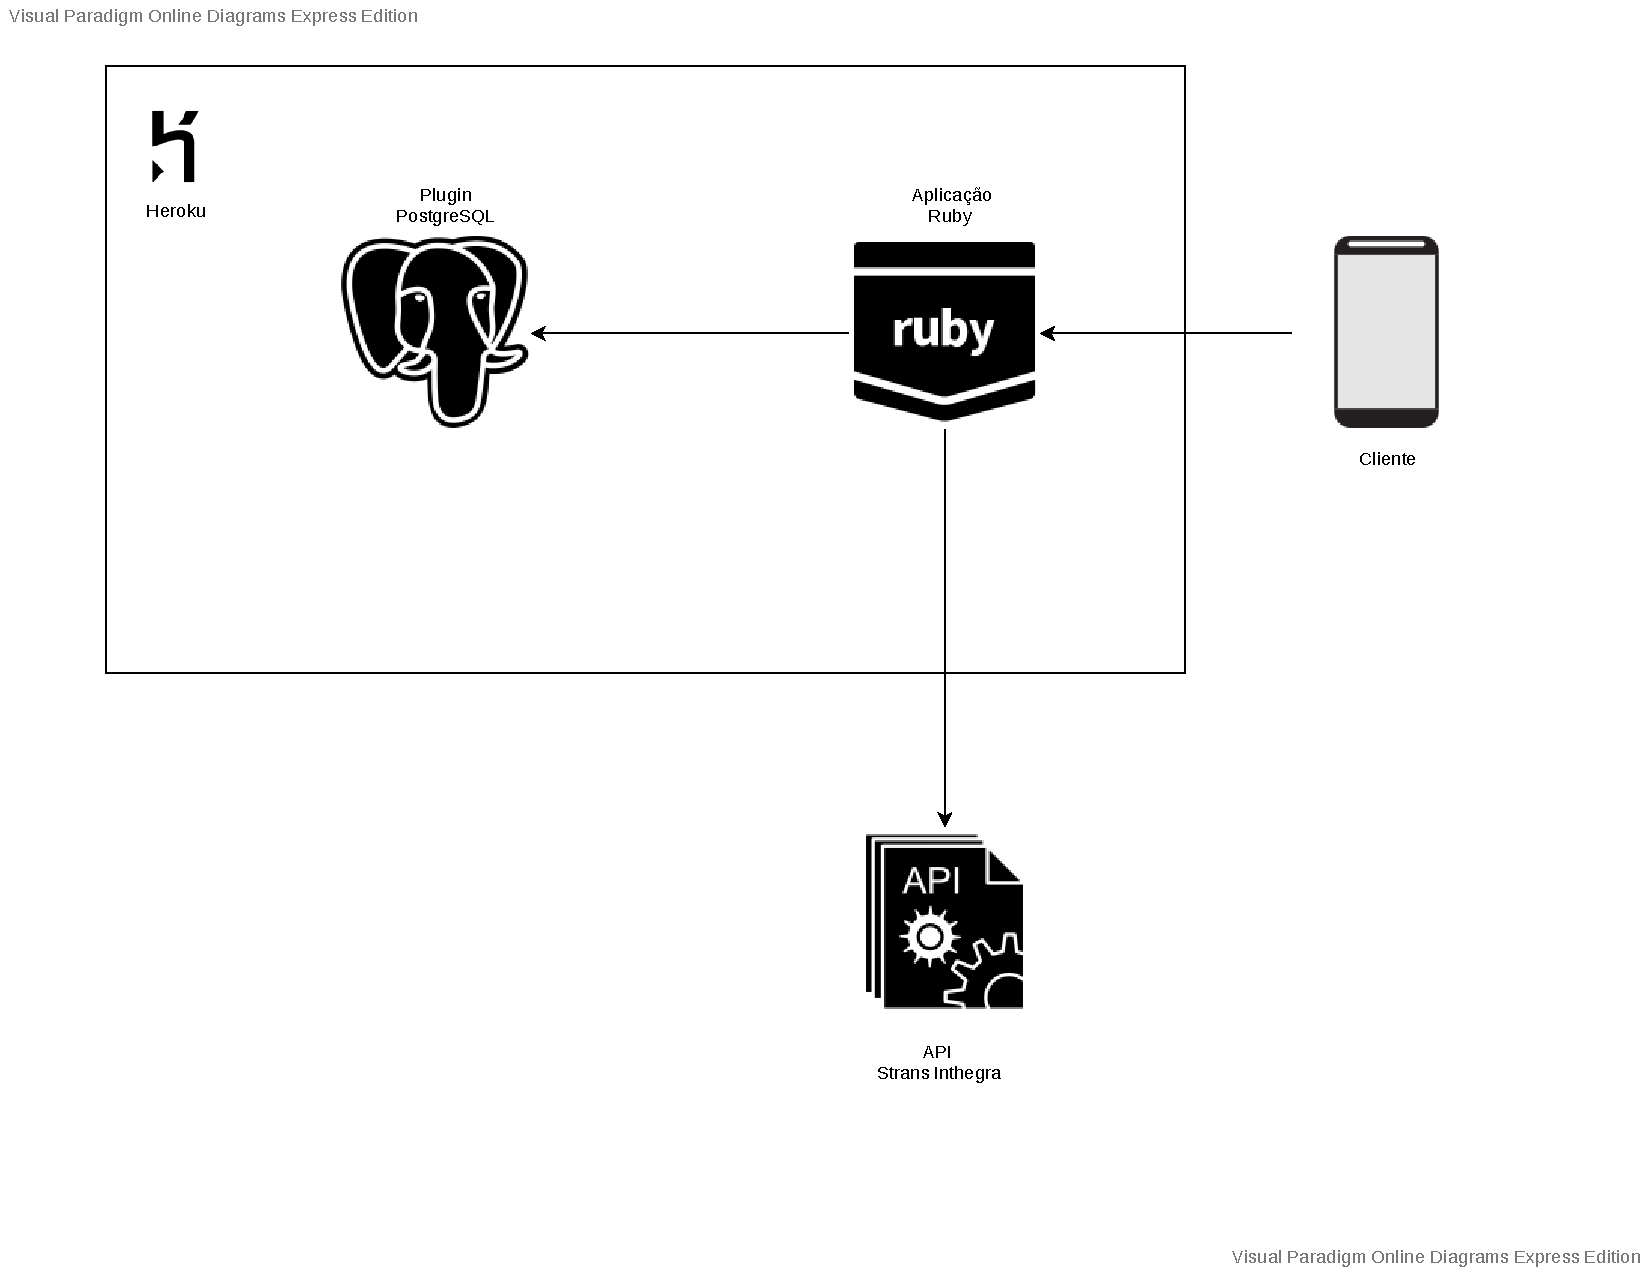
\includegraphics[scale=0.6]{imagens/arquitetura-sb.pdf}
\end{figure}


\section{Diagrama de Entidades-Relacionamentos} \label{sec:modelagem:der}

Na figura \ref{fig:uml_der} podemos ver a estrutura lógica usada como base para o banco de dados. A maioria representam 
as entidades detalhadas anteriormente no Diagrama de Classe, com exceção da entidade schema\_migrations, que é utilizada pelo 
framework Active Record para armazenar o histórico de migrações utilizadas por ele.

\begin{figure}[H]
  \caption{\label{fig:uml_der}Diagrama entidade-relacionamento}
  \centering
  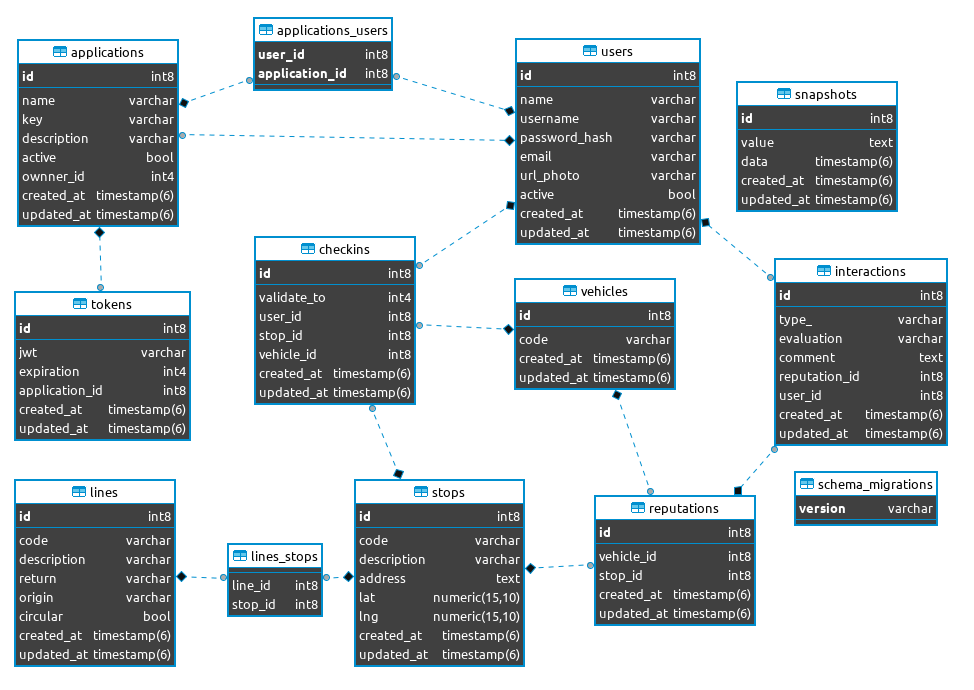
\includegraphics[scale=0.5]{imagens/diagramaer-sb.png}
\end{figure}

\section{API REST} \label{sec:modelagem:classe}

Como já descrito, essa plataforma que utiliza o conceito de API REST e toda a comunição é feita por meio 
de métodos http, que são organizados sematicamente com base em resources, abaixo serão descritos os resources
bem como os metodos que são disponíveis na API da plataforma. Toda a transmissão de dados será feita utilizand 
o padrão JSON, assim sendo o corpo das requisições bem como das resposta da api serão texto obedecendo as 
regras desse padrão amplamente difundido na WEB.  

Todos as requisições a api deve ser feitas utilizando o cabeçalho de "Authorization" com 
o token de autenticação recuperado de "auth/login", intuitivamente essa chamada é a única que 
não é obrigatório a inclusão do cabeçalho de autenticação. 

Por padrão os resources abaixo retornam os seguintes codigos http, para cada situação descrita.

\begin{lista}
  \item \textbf{200}: Solicitação executada com sucesso.
  \item \textbf{403}: Token inválido ou não enviado.
  \item \textbf{404}: O path não foi encontrado ou não existe entidade com id/código especificado.
  \item \textbf{415}: Solicitação fora do formato esperado pela API.
  \item \textbf{500}: Erro interno do servidor.
\end{lista}

A url base da API é https://starbus-v2.herokuapp.com/v2/ que é seguida pelo resources detalhados a seguir.

\subsection{/auth}

Responsável pelos dados de autenticação na platafroma. Basicamente retorna o token de acesso que
deve ser utilizando nas próximas requisições, e returna dados sobre o usuário autenticado com o 
com o token utilizado. 

\begin{table}[htbp]
	\scriptsize
	\centering
	\begin{tabular}{|l|l|l|}
		\hline \textbf{Método} & \textbf{Caminho} & \textbf{Descrição} \\ 
    \hline POST   & /login    & Autentica o usuário e retorna o token que será utilizado posteriomente \\
    \hline GET   & /sesion    & Retorna os dados o usuário logado com token passado \\
		\hline 
	\end{tabular}
	\caption{Resource Auth}
	\label{tab:resources}
\end{table}


\subsection{/applications}

Gerenciamento de aplicações da plataforma que só pode ser feito pelo usuário que possui as aplicações. Assim 
cada usuário gerencia suas próprias aplicações. 

\begin{table}[htbp]
	\scriptsize
	\centering
	\begin{tabular}{|l|l|l|}
		\hline \textbf{Método} & \textbf{Caminho} & \textbf{Descrição} \\ 
    \hline POST   & /    & Cria uma nova Application com os dados passados \\
		\hline GET    & /    & Retorna todas as Applications \\
		\hline PUT    & /:id & Atualiza a Application com id espeficicado, como os dados passados \\
		\hline GET    & /:id & Retorna a Application com o id espeficicado \\
		\hline DELETE & /:id & Desativa a Application com o id espeficicada \\
		\hline 
	\end{tabular}
	\caption{Resource Applications}
	\label{tab:resources}
\end{table}

\subsection{/users}

Gerenciamento de usuários.

\begin{table}[htbp]
	\scriptsize
	\centering
	\begin{tabular}{|l|l|l|}
		\hline \textbf{Método} & \textbf{Caminho} & \textbf{Descrição} \\ 
    \hline POST   & /    & Cria uma nova User com os dados passados \\
		\hline GET    & /    & Retorna todas as Users \\
		\hline PUT    & /:id & Atualiza a User com id espeficicado, como os dados passados \\
		\hline GET    & /:id & Retorna a User com o id espeficicado \\
		\hline DELETE & /:id & Desativa a User com o id espeficicado \\
		\hline 
	\end{tabular}
	\caption{Resource Users}
	\label{tab:resources}
\end{table}

\subsection{/lines}

As Linhas disponíveis na aplicação são fornecidas e gerenciadas pela API Strans, assim o Starbus
não faz o gerenciamento dessas linhas, ele apenas carrega tais linhas de sua fonte. O resource abaixo
carrega tais linhas e oferece algumas consultas as linhas na base.

\begin{table}[htbp]
	\scriptsize
	\centering
	\begin{tabular}{|l|l|l|}
    \hline \textbf{Método} & \textbf{Caminho} & \textbf{Descrição} \\
    \hline POST   & /load & Carregas as linhas a partir da API Strans \\
    \hline GET    & /     & Retorna todas as Lines \\
    \hline GET    & /?codigos[]=:codigo  & Retorna as Lines com os códigos espeficicados \\
    \hline GET    & /:codigo/vehicles/  & Retorna os Vehicles com na rota da linha com o código passado \\
		\hline 
	\end{tabular}
	\caption{Resource Lines}
	\label{tab:resources}
\end{table}

\subsection{/vehicles}

Assim como as linhas a Lines, Veihcles não são gerenciados pelo Starbus, a cada consulta na Strans a 
plataforma se o Veihcle já está cadastrado em sua base, se não ela cadastra. Sendo assim, esse  resource
retorna simplesmente os Veihcles rodando no momento da requisição.

\begin{table}[htbp]
	\scriptsize
	\centering
	\begin{tabular}{|l|l|l|}
		\hline \textbf{Método} & \textbf{Caminho} & \textbf{Descrição} \\ 
    \hline GET    & /  & Retorna todas as Vehicles rodando no sistema nesse momento \\
    \hline GET    & /:codigo  & Retorna o Vehicle rodando no sistema com sua posição no momento \\
    \hline POST   & /:codigo/checkin & Realiza o Checkin na Stop com o código passado \\
    \hline 
	\end{tabular}
	\caption{Resource Vehicles}
	\label{tab:resources}
\end{table}

% \clearpage

\subsection{/stops}

Stops também não são gerenciados pela plataforma e são carregados por quando as Lines são carregadas,
a cada Line carrega são automaticamente salvos as paradas associadas a ela.

\begin{table}[htbp]
	\scriptsize
	\centering
	\begin{tabular}{|l|l|l|}
		\hline \textbf{Método} & \textbf{Caminho} & \textbf{Descrição} \\ 
    \hline GET    & /               & Retorna todas as Stops do sistema \\
		\hline GET    & /:codigo/lines  & Retorna todas as Lines de uma Stop com o código espeficicado \\
    \hline GET    & /closes/?lat=:lat\&long=:long  & Retorna todas as Stops proximas a localização passadas por meio de lat e long \\
    \hline POST   & /:code/checkin & Realiza o Checkin na Stop com o código passado. \\
    \hline  
	\end{tabular}
	\caption{Resource Lines}
	\label{tab:resources}
\end{table}

\subsection{/interations}

Esse resource o é possível registrar as avaliações dos usuários sobre dois componentes do sistem de transpote píblico, 
paradas de ônibus e veículos. 

\begin{table}[htbp]
	\scriptsize
	\centering
	\begin{tabular}{|l|l|l|}
		\hline \textbf{Método} & \textbf{Caminho} & \textbf{Descrição} \\ 
    \hline GET    & /:criterio/vehicle/:codigo  & Retorna a User com o id espeficicado \\
		\hline GET    & /:criterio/stop/:codigo     & Retorna todas as Users \\
    \hline POST   & /:criterio/vehicle/:codigo  & Cria uma nova User com os dados passados \\
    \hline POST   & /:criterio/stop/:codigo     & Cria uma nova User com os dados passados \\
		\hline 
	\end{tabular}
	\caption{Resource Interactions}
	\label{tab:resources}
\end{table}

Abaixo são listados os critérios que são utilizados para avaliar essas entidades, que nos 
caminhos são representados pelo parametro ":criterio".

\begin{lista}
  \item \textbf{accessibility}: Acessibilidade de acesso para pessoas dificuldade de locomoção.
  \item \textbf{comfort}: Conforto para o usuário.
  \item \textbf{safety}: Segurança, tanto no aspecto de uso como de segurança pública.
  \item \textbf{state}: Estado de conservação.
\end{lista}

Par cada um dos critérios a acima o usuário pode associar uma avaliação listada a abaixo para a entidade 
que está avaliando que é especificada pelo ":codigo" da entidade. 

\begin{lista}
  \item \textbf{bad}: Ruim, longe de ser o ideal. 
  \item \textbf{regular}: Regular, atende as necessidades do usuário.
  \item \textbf{good}: Muito bom, não deixando a desejar em nenhum aspecto.
\end{lista}

\clearpage



